\chapter{Mécanique}

\newpage

\section{Le Petit Prince : satellisation d'une pomme $\bullet\bullet\circ\circ$}

On se place à la surface d'une planète de rayon $R$ et de champ gravitationnel $g$. On envoie une pomme avec une vitesse $v_0$ purement horizontale et on négligera les frottements de l'air.

\begin{enumerate}
\item En supposant la planète localement plane, déterminer la hauteur d$z$ dont est tombée la pomme après avoir parcouru une longueur d$x$ dans le plan horizontal. % d$z=\dfrac{g(\mathrm{d}x)^2}{2{v_0}^2}$
\item Après une distance horizontale d$x$, de combien le sol de la planète est-il descendu ? On pourra utiliser les formules pour les petits angles : $\tan\theta\simeq \theta$, $\sin\theta\simeq \theta$ et $\cos\theta\simeq 1-\theta^2/2$. % Il faut penser à la rotondité de la Terre qui n'est donc pas parfaitement plane localement : d$h=R-R\cos(\mathrm{d}\theta)=R(\mathrm{d}\theta)^2/2=(\mathrm{d}x)^2/2R$
\item En déduire qu'il existe une certaine vitesse $v_0$ pour laquelle la pomme va revenir à son point de départ. % v_0=\sqrt{GM/R}$
\end{enumerate}

\newpage

\begin{correction}

\begin{enumerate}
\item La planète étant supposée parfaitement plane, on peut commencer par calculer l'équation du mouvement de la pomme. Soumise à la seule force de pesanteur, on obtient :

\begin{align*}
	\left\lbrace
\begin{array}{ccc}
 x(t) =  v_0t+x_0 \\
 z(t) = -\frac{1}{2}gt^2+z_0 \\
\end{array}\right.
\end{align*}
En supposant que $x_0$ et $z_0$ sont les coordonnées de la position initiale. On obtient donc l'équation de la trajectoire :
\begin{align*}
	z(x) = -\frac{g(x-x_0)^2}{2v_0^2}+z_0
\end{align*}

Lorsque la pomme avance de $dx$ par rapport à sa position initiale $x_0$, elle descend de $z_0$ à $z_0+dz$ :
\begin{align*}
	z(x_0+dx)=z_0+dz=-\frac{gdx^2}{2v_0^2}+z_0
\end{align*}
Donc $dz=-\frac{gdx^2}{2{v_0}^2}$.

\item Il faut penser à la rotondité de la Terre qui n'est donc pas parfaitement plane localement : d$h=R-R\cos(\mathrm{d}\theta)=R(\mathrm{d}\theta)^2/2=(\mathrm{d}x)^2/2R$.

\item Si la vitesse initiale est suffisament grande, la chute de la pomme est compensée par le fait que le sol "s'abaisse" en même temps à cause de la rotondité, cad $dh=-dz$, soit $v_0=\sqrt{gR}=\sqrt{GM_T/R}$.

\item Si la pomme revient à son point de départ, c'est que la trajectoire est supposée circulaire, avec $R$ constant. On peut effectuer un PFD sur la pomme en coordonnées cylindriques, et trouver à partir de la projection sur $\vec{e}_r$ :

\begin{align*}
 -mR\dot{\theta}^2 =  -\frac{GmM_T}{R^2} 
\end{align*}
Soit $v_0=R\dot{\theta}=\sqrt{GM_T/R}$.
\end{enumerate}

\end{correction}

\newpage

\section{Projectile lancé à la verticale $\bullet\circ\circ\circ$}

On tire un petit projectile à la verticale, avec une vitesse initiale $v_0$. Le problème est de calculer son altitude $z$ en fonction du temps, en tenant compte de la gravité et de la résistance de l'air. Comme l'objet est petit, on supposera que la résistance de l'air est proportionnelle à la vitesse et que la force de résistance est $m\gamma v$, $m$ étant la masse de l'objet, $v$ sa vitesse et $\gamma$ une constante. Nous supposerons que la force de gravité est constante (on néglige sa variation en fonction de l'altitude). On adoptera comme origine la position du tir ($z=0$) et on supposera que le mouvement ne se produit que dans la direction $z$.

\begin{enumerate}
\item Soit $v(t)$ la composante en $z$ de la vitesse du projectile. \'{E}crivez l'équation différentielle que doit satisfaire $v(t)$ en fonction du temps, d'après la deuxième loi de Newton.
\item Résoudre cette équation différentielle avec la condition initiale $v(0)=v_0$.
\item Exprimer maintenant l'altitude $z$ en fonction du temps.
\item Calculer l'altitude maximale atteinte par le projectile ($z_\mathrm{max}$), en fonction des paramètres $v_0$, $g$ et $\gamma$.
\item Exprimer le résultat de la question précédente ($z_\mathrm{max}$) dans les limites de très faible résistance ($\gamma \rightarrow 0$) et de très forte résistance ($\gamma \rightarrow \infty$). Quelles modifications mineures devrait-on apporter à l'équation différentielle trouvée première question pour retrouver ces résultats plus simplement ?

\end{enumerate}

\newpage

\begin{correction}

\begin{itemize}
\item Rien de bien difficile, en notant $v=\dot{z}$ :

\begin{align*}
	m\dot{v}=-\gamma mv-mg
\end{align*}

\item
La solution de cette équation est :
\begin{align*}
	v(t) = \left(v_0+\frac{g}{\gamma} \right)\exp\left(-\gamma t\right)-\frac{g}{\gamma}  
\end{align*}

\item On intègre l'expression de la vitesse précédente. On trouve :

\begin{align*}
	z(t) = \frac{1}{\gamma}\left(v_0+\frac{g}{\gamma} \right) \left(1-\exp(-\gamma t) \right) -\frac{g}{\gamma}t
\end{align*}
\item L'altitude maximale correspond à l'instant $t_0$ où la vitesse s'annule : $v(t_0)=0$, soit $t_0 = \frac{1}{\gamma}\ln\left(\frac{1+v_0\gamma}{g} \right) $. On a donc :
$z_\mathrm{max}=\frac{v_0}{\gamma}-\frac{g}{\gamma^2}\ln\left( 1+\frac{\gamma v_0}{g}\right).$

\item Dans le cas où $\gamma\rightarrow0$, $z_\mathrm{max}\rightarrow\frac{v_0}{\gamma}-\frac{g}{\gamma^2}\frac{\gamma v_0}{g}+\frac{g}{2\gamma^2}\frac{\gamma^2 v_0^2}{g^2}=\frac{ v_0^2}{2g}$ en utilisant $\ln(1+x)\simeq 1+x-x^2/2$. Cela correspond à une chute libre ne l'absence de frottement. 

Dans le cas où $\gamma\rightarrow0$, $z_\mathrm{max}\rightarrow\frac{v_0}{\gamma}$

\end{itemize}

\end{correction}

\newpage

\section{Paramètre d'impact $\bullet\bullet\circ\circ$}

Une météorite arrive depuis l'infini vers la Terre avec une vitesse à l'infini $\vec{v}_0$. La Terre a une masse $M_T$ et un rayon $R_T$. On note $b$ le paramètre d'impact comme indiqué sur la figure ci-dessous. L'objectif de ce problème est de déterminer la valeur minimale de $b$ pour laquelle la météorite évite la collision avec la Terre.

\begin{figure}[h]
\centering
  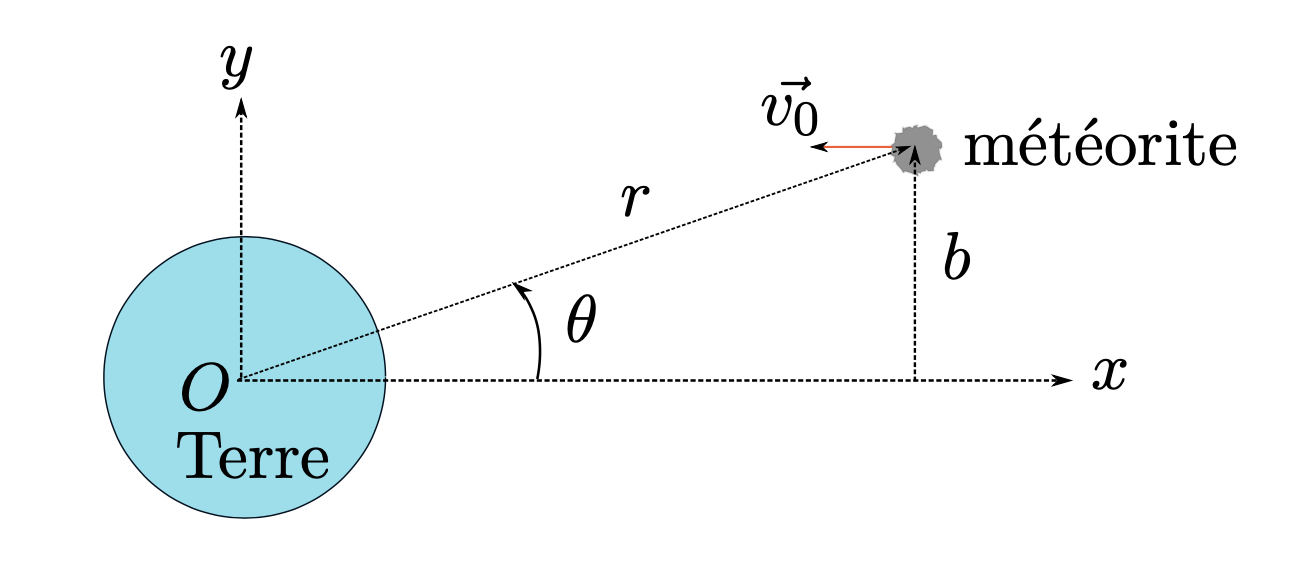
\includegraphics[scale=0.4]{meca_parametre_impact.png}
\end{figure}

\begin{enumerate}
\item La météorite n'est soumise qu'à la force gravitationnelle de la Terre. Déterminer la nature de sa trajectoire. Montrer que le mouvement est plan et déterminer une relation entre $r$ et $\dot{\theta}$.
\item On note $N$ le point de la trajectoire où la distance qui sépare la météorite de la Terre est la plus petite. Montrer qu'en $N$, la vitesse est uniquement suivant $\vec{u}_\theta$. Déterminer une relation entre $v_N$ au point $N$, la distance $ON$, $b$ et $v_0$.
\item En utilisant la conservation de l'énergie, montrer la relation :
$$
0=r^2_\mathrm{min}v_0^2+2GM_Tr_\mathrm{min}-v_0^2b^2.
$$
\item En déduire l'expression minimale $b_c$ du paramètre d'impact telle que pour $b<b_c$, la météorite frappe la Terre et pour $b>b_c$, la météorite évite la Terre. On pourra exprimer le résultat en fonction de la vitesse de libération $v_\mathrm{lib}$.
\end{enumerate}

\newpage

\begin{correction}

\begin{enumerate}
\item La météorite n'est soumise qu'à la gravitation, qui est une force centrale. On peut donc utiliser la conservation du moment cinétique (car le moment des forces est nul). Comme le moment se converve, il est dirigé ortohogonalement au plan délimité par $\vec{r_0}$ et $\vec{v_0}$ tout le long de la trajectoire. Le mouvement reste donc conscrit à ce plan.

D'autre part, on a par la conservation du moment :
\begin{align*}
	\vec{\sigma}_O(M)=m\vec{r}\wedge\vec{v}=-mr_0v_0sin(\theta_0)=-mbv_0
\end{align*}

Et d'autre part, $\vec{v}=\dot{r}\vec{e}_r+r\dot{\theta}\vec{e}_\theta$, donc $\vec{\sigma}_O(M)=r^2\dot{\theta}=-mbv_0$.


\item La distance $ON$ entre la météorite et la terre correspond à la coorodnnée $r$. Lorsque celle-ci est minimale, on a nécéssairement $\dot{r}=0$. La vitesse s'exprime donc $\vec{v}=\dot{r}\vec{e}_r+r\dot{\theta}\vec{e}_\theta=r\dot{\theta}\vec{e}_\theta$.

A ce point, le moment cinétique est $\vec{\sigma}_O=ON\cdot v_N$. Par conservation du moment on a alors :
\begin{align*}
	ON\cdot v_N=bv_0
\end{align*}

\item L'énergie potentielle de gravitation s'écrit $E_p=-GM_Tm/r^2$. L'énergie mécanqiue totale du système est égale au point $N$ et à l'infini (lorsque la météorite arrive à la vitesse $v_0$), alors :
\begin{align*}
	\frac{1}{2}mv_N^2-\frac{GM_Tm}{r_N}
\end{align*}
$$
0=r^2_\mathrm{min}v_0^2+2GM_Tr_\mathrm{min}-v_0^2b^2.
$$
\item En déduire l'expression minimale $b_c$ du paramètre d'impact telle que pour $b<b_c$, la météorite frappe la Terre et pour $b>b_c$, la météorite évite la Terre. On pourra exprimer le résultat en fonction de la vitesse de libération $v_\mathrm{lib}$.

\end{enumerate}

\end{correction}

\newpage

\section{Piège de Penning $\bullet\bullet\bullet\circ$}

A l'aide d'un dispositif approprié, on créé dans une région de l'espace au voisinage d'un point $O$ un champ électrique défini en coordonnées carthésiennes par :
\begin{align*}
	\vec{E}=\frac{U_0}{2R^2}\left(-x\vec{e}_x-y\vec{e}_y+2z\vec{e}_z \right) 
\end{align*}
Un électron de masse $m$ et de charge $e$ se meut dans la région située autour du point $O$.

\begin{enumerate}

	\item Montrer que le point $O$ est une position d'équilibre pour l'éléctron. Discuter de la stabilité selon les directions. On introduira $\omega_z^2=eU_0/mR^2$.

 \item Pour stabiliser la trajectoire de l'électron, on supperpose au champ électrique un champ magnétique uniforme et constant $\vec{B}=B_0\vec{e}_z$. On définit $\omega_c=eB_0/m$. 

\begin{enumerate}

		\item Montrer que le mouvement suivant $\vec{e}_z$ est inchangé.
		
		\item Pour le mouvement dans le plan $(xOy)$, montrer que l'électron n'est piégé que si $B_0$ est supérieur a une certaine valeur $B_c$, à déterminer en fonction des données de l'exercice. On utilisera le changement de variable : $\rho = x+iy$.
		
		\item Résoudre l'équation en $\rho$ pour le cas $B_0\gg B_c$, sans chercher à mettre en évidence les constante d'intégration, mais en mettant en évidence deux pulsations, l'une voisine de $\omega_c$, notée $\omega_c'$, et une autre notée $\omega_m$, appelée pulsation magnétique. 

\end{enumerate}
		
\end{enumerate}

\newpage

\begin{correction}

\begin{enumerate}

	\item On applique le principe fondamental de la dynamique à l'électron :
\begin{align*}
	\left\lbrace
\begin{array}{ccc}
 m\ddot{x} &=&  e\frac{U_0}{2R^2}x \\
 m\ddot{y} &=& e\frac{U_0}{2R^2}y \\
 m\ddot{z} &= & -e\frac{U_0}{R^2}z \\
\end{array}\right.
\end{align*}
La position est bien une position de stabilité : les forces appliquée en ce point sont nulles. Néanmoins, ce n'est pas une position stable en $x$ ou en $y$ car la solution est exponentielle. Le mouvement est stable uniquement sur $z$, avec une pulsation $\omega_z=eU_0/mR^2$.

\item

\begin{enumerate}

		\item Le PFD devient :
		
\begin{align*}
	\left\lbrace
\begin{array}{ccc}
 \ddot{x} &=&  \frac{\omega_z^2}{2}x - \omega_c\dot{y}\\
 \ddot{y} &=& \frac{\omega_z^2}{2}y + \omega_c\dot{x} \\
 \ddot{z} &= & -\omega_z^2z \\
\end{array}\right.
\end{align*}

Le mouvement selon $z$ est bien inchangé. 

		\item En multipliant la seconde première ligne par $i$, puis en sommant ces deux lignes, on obtient :
		\begin{align*}
 \ddot{\rho} - \frac{\omega_z^2}{2}\rho - i\omega_c\dot{\rho}=0\\
\end{align*}
		
		Le déterminant de l'équation caractéristique est $\Delta=2\omega_z^2-\omega_c^2$. Le mouvement est stable uniquement si $\Delta>0$, cad si $B_0>B_c=\sqrt{2mU_0/eR^2}$.
		
		\item Les solutions de l'équation caractéristiques sont :
		\begin{align*}
			r=i\frac{\omega_c}{2}\left( 1 \pm\sqrt{1- \frac{2\omega_z^2}{\omega_c^2}}\right) 
		\end{align*}
		
		Les pulsations caractéristiques sont donc $\omega_\pm=\frac{\omega_c}{2}\left( 1 \pm\sqrt{1- \frac{2\omega_z^2}{\omega_c^2}}\right)$. Dans le cas où $B_0\gg B_c$, $\omega_c\gg\omega_z$ et on peut donc écrire :
		\begin{align*}
			\omega_+&=\frac{\omega_c}{2}\left( 1 +\frac{\omega_z^2}{2\omega_c^2}\right)= \omega_c'\\
			\omega_-&=\frac{\omega_z^2}{2\omega_c}=\omega_m
		\end{align*}
		
		La solution est donc :
		\begin{align*}
			\rho(t)=Ae^{i\omega_c'}t+Be^{i\omega_mt}
		\end{align*}
		
		L'équation de la trajectoire est donnée par $x(t)=\mathrm{Re}(\rho(t))$ et $y(t)=\mathrm{Im}(\rho(t))$.

\end{enumerate}
		
\end{enumerate}

\end{correction}

\newpage

\section{Tir à grande distance $\bullet\bullet\circ\circ$}

Dans le jeu \textit{Call of Duty 4 : Modern Warfare}, le joueur prend le rôle d'un tireur d'élite devant abattre une cible située à une distance $d=$897m à l'aide d'un fusil de précision, qui tire un projectile à une vitesse $v_0=850$m.s$^{-1}$. Le tir s'effectue depuis le dernier étage d'un immeuble d'une hauteur $H=30$m, la cible se trouvant plein nord par rapport au tireur. La scène se situe en Russie, à une latitude $\lambda=45^\circ$. Le coéquipier du joueur précise, avant le tir, qu'il faut tenir compte de l'effet de Coriolis et l'on souhaite vérifier cette affirmation.

On définit $R=(O,x,y,z)$ le repère situé au pied de l'immeuble où se trouve le joueur, avec l'axe $\vec{e}_x$ dirigé vers l'est et l'axe $\vec{e}_y$ se dirigeant vers le nord. On notera $\vec{\Omega}_T$ le vecteur rotation de la terre. On supposera que les frottements de l'air sont négligés.

\begin{enumerate}

	\item Montrer que les équations du mouvement dans le référentiel $R$ de la balle une fois que le tireur fait feu s'écrivent :
	\begin{align*}
        \ddot{x}=&2\Omega_T(\sin\lambda\dot{y}-\cos\lambda\dot{z})\\ 
        \ddot{y}=&-2\Omega_T\sin\lambda\dot{x} \\
        \ddot{z}=&-g+2\Omega_T\cos\lambda\dot{x}
	\end{align*}
	
	\item Déterminer la solution sur $x(t)$ sans préciser les variables d'intégration.
	
	\item Donner une estimation du temps de vol avant impact $t_{impact}$ puis simplifier les équations du mouvement, les résoudre.
	
	\item Que pensez-vous de l'affirmation du coéquipier ? Quel est l'écart $\vec{\varepsilon}$ de la balle par rapport à si celle-ci avait une trajectoire parfaitement rectiligne ?

\end{enumerate}

\newpage

\section{Tir à grande distance $\bullet\bullet\bullet\bullet$}

Dans le jeu \textit{Call of Duty 4 : Modern Warfare}, le joueur prend le rôle d'un tireur d'élite devant abattre une cible située à une distance $d=$897m à l'aide d'un fusil de précision, qui tire un projectile à une vitesse $v_0=850$m.s$^{-1}$. Le tir s'effectue depuis le dernier étage d'un immeuble d'une hauteur $H=30$m, la cible se trouvant plein nord par rapport au tireur. La scène se situe en Russie, à une latitude $\lambda=45^\circ$. Le coéquipier du joueur précise, avant le tir, qu'il faut tenir compte de l'effet de Coriolis et l'on souhaite vérifier cette affirmation. On définit $R=(O,x,y,z)$ le repère situé au pied de l'immeuble où se trouve le joueur, avec l'axe $\vec{e}_x$ dirigé vers l'est et l'axe $\vec{e}_y$ se dirigeant vers le nord. On notera $\vec{\Omega}_T$ le vecteur rotation de la terre. On supposera que les frottements de l'air sont négligés.

Que pensez-vous de l'affirmation du coéquipier ? Quel est l'écart $\vec{\varepsilon}$ de la balle par rapport à si celle-ci avait une trajectoire parfaitement rectiligne ? On pourra donner une estimation du temps de vol avant impact $t_{impact}$ pour simplifier les équations du mouvement.

\newpage

\begin{correction}

On note $R'$ le référentiel du tireur, sur la terre en rotation, et $R$ le référentiel galiléen, ne tournant pas avec la terre. Le vecteur rotation de $R'/R$ s'écrit $\vec{\Omega}=\Omega_T\cdot(\cos\lambda\vec{e}_y+\sin\lambda\vec{e}_z)$ et on note le vecteur vitesse dans $R'$ : $\vec{v}=\dot{x}\vec{e}_x+\dot{y}\vec{e}_y+\dot{z}\vec{e}_z$. Une fois sortie du canon, la balle est uniquement soumise à la gravité et à la force de Coriolis (la force d'inertie d'entrainement est comprise dans $g$). Cette dernière s'écrit :
	\begin{align*}
		\vec{F}_c&=-2m\vec{\Omega}\wedge\vec{v} \\
		&=2m\Omega_T\left\lvert 
      \begin{matrix} 
        &\sin\lambda\dot{y}-\cos\lambda\dot{z}\\ 
        &-\sin\lambda\dot{x} \\
         &\cos\lambda\dot{x}
      \end{matrix}  
    \right.
	\end{align*}

Le PFD donne donc :
	\begin{align*}
        \ddot{x}=&2\Omega_T(\sin\lambda\dot{y}-\cos\lambda\dot{z})\\ 
        \ddot{y}=&-2\Omega_T\sin\lambda\dot{x} \\
        \ddot{z}=&-g+2\Omega_T\cos\lambda\dot{x}
	\end{align*}
Ces équations sont toutes intégrables. On intègre la deuxième et la troisième :
	\begin{align*}
        \ddot{x}=&2\Omega_T(\sin\lambda\dot{y}-\cos\lambda\dot{z})\\ 
        \dot{y}=&-2\Omega_T\sin\lambda x + \dot{y}_0 \\
        \dot{z}=&-gt+2\Omega_T\cos\lambda x + \dot{z}_0
	\end{align*}
Et on injecte dans la première équation sur $x$, et en simplifiant les $\cos^2+\sin^2$ : 
\begin{align*}
	\ddot{x}+4\Omega_T^2x=2\Omega_T(\sin\lambda\dot{y}_0-\cos\lambda\dot{z}_0)+2\Omega_T\cos\lambda gt
\end{align*}
	Cette équation est soluble : elle du genre $\ddot{x}+\omega_0^2=a+bt$. Néanmoins, la solution homogène en $\cos$ et $\sin$ n'est pas très intéressante : la période est celle de la journée terrestre, elle correspond en fait à ce que la balle fasse le tour de la Terre et revienne à sa position... Et en effet, comme $\Omega_T\simeq7,2\times10^{-7}$rad/s, on peut commencer à garder uniquement les termes en $\Omega_T^2$ d'ordre 1 devant les autres termes. On a donc, après simplification :
	\begin{align*}
        x(t)=& \frac{1}{3}\Omega_T\cos\lambda t^3+\Omega_T(\sin\lambda\dot{y}_0-\cos\lambda\dot{z}_0)t^2+\dot{x}_0t\\ 
        y(t)=&-\Omega_T\sin\lambda \dot{x}_0t^2 + \dot{y}_0t \\
        z(t)=&-\frac{1}{2} gt^2+\Omega_T\cos\lambda \dot{x}_0t^2 + \dot{z}_0t+z_0
	\end{align*}	
On a donc les équations du mouvement. Néanmoins, cela reste encore un peu dur de conclure. On peut encore essayer de simplifier certains termes, en utilisant l'estimation du temps de vol et la vitesse initiale. Le temps de vol, estimé à 1s environ, permet de comparer le premier et le deuxième terme dans l'équation sur $x(t)$ : $\frac{1}{3}gt^3\ll\dot{y}_0t^2$, durant tout le temps de vol, comme $\dot{y}_0\simeq 850$. D'autre part, comme le tir est dirigé plein nord, on a $\dot{x}_0=0$. On a alors :
	\begin{align*}
        x(t)=& \Omega_T(\sin\lambda\dot{y}_0-\cos\lambda\dot{z}_0)t^2\\ 
        y(t)=&\dot{y}_0t \\
        z(t)=&-\frac{1}{2} gt^2 + \dot{z}_0t+z_0
	\end{align*}	
Et en notant $\alpha$ l'angle que fait le tireur entre l'horizontale et la direction du canon (comme il est situé sur un immeuble, il y a un léger dénivellé entre lui et sa cible), on a :
	\begin{align*}
        x(t)=& v_0\Omega_T\sin(\lambda+\alpha)t^2\\ 
        y(t)=&v_0\cos(\alpha)t \\
        z(t)=&-\frac{1}{2} gt^2 -v_0\sin(\alpha)t+z_0
	\end{align*}	
Finalement, on se retrouve avec globalement une chute libre classique, si ce n'est un terme de déviation uniquement sur $x$, vers l'est. Si la balle partait de manière parfaitement rectiligne, sa trajectoire serait (soumise à aucune force) :
	\begin{align*}
        x'(t)=& 0\\ 
        y'(t)=&v_0\cos(\alpha)t \\
        z'(t)=& -v_0\sin(\alpha)t+z_0
	\end{align*}	
La dévitation est donc $\vec{\varepsilon	}=v_0\Omega_T\sin(\lambda+\alpha)t^2\vec{e}_x-\frac{1}{2} gt^2\vec{e}_z$. Pour un temps de vol d'environ 1 seconde, on trouve que :
\begin{align*}
	\vec{\varepsilon}=-0,5\vec{e}_z+0,04\vec{e}_x
\end{align*}
La balle est déviée de seulement 4cm vers l'est : Coriolis est donc négligeable. Par contre, il faut tenir compte du poids dont l'effet est bien plus marqué. 
	
\end{correction}

\newpage

\section{Frottement d'une corde et d'une poutre en bois $\bullet\bullet\circ\circ$}

Une corde est enroulée autour d'une poutre en bois de section circulaire, d erayon $R$, entre les angles $\theta_1$ et $\theta_2$. Au-delà de ces angles, la corde n'est plus en contact avec le bois et est soumise aux tensions $T_1$ et $T_2$ de part et d'autre de ses extrémités. Le coeffcient de forttement entre la corde et le bois est $f=0,5$. On note $T(\theta)$ la tension dans la corde à un angle $\theta$, c'est-à-dire la force qui s'exerce au sein de la corde.

\begin{figure}[h]
\centering
  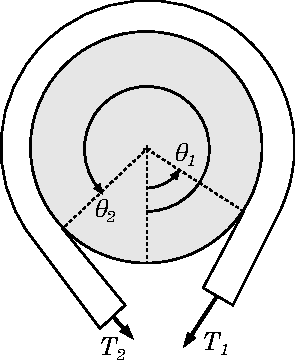
\includegraphics[scale=0.8]{meca_corde.pdf}
\end{figure}

\begin{enumerate}

	\item Montrer que la réaction normale $dR_N$ de la poutre sur un élément de longueur de corde $Rd\theta$ vérifie la relation suivante :
	\begin{align*}
		dR_N+T(\theta)d\theta=0
	\end{align*}
	
	\item Montrer que la réaction tangentielle $dR_T$ de la poutre sur un élément de longueur de corde $Rd\theta$ vérifie la relation suivante :
	\begin{align*}
		-dR_T+T(\theta+d\theta)-T(\theta)=0
	\end{align*}
	
	\item En déduire une équation différentielle sur la tension $T(\theta)$ et l'intégrer.
	
	\item Pour attacher son cheval, un cow-boy enroule tout simplement la longe de son cheval de plusieurs tour autour d'une poutre en bois de section ronde, puis laisse l'extrémité libre, soumise à son propre poids (environ 100g). Combien de tours le cow-boy doit-il effectuer pour qu ele cheval ne puisse pas dérouler la corde ?
	
\end{enumerate}

\textit{Indications} : la force maximale que peut développer un cheval est équivalent à une tonne ; le coefficient de frottement entre la corde et le bois est $f=0,5$.

\newpage

\section{Frottement d'une corde et d'une poutre en bois $\bullet\bullet\bullet\circ$}

Pour attacher son cheval, un cow-boy enroule tout simplement la longe de son cheval de plusieurs tour autour d'une poutre en bois de section ronde, puis laisse l'extrémité libre, soumise à son propre poids (environ 100g). Combien de tours le cow-boy doit-il effectuer pour qu ele cheval ne puisse pas dérouler la corde ?

\textit{Indications} : la force maximale que peut développer un cheval est équivalent à une tonne ; le coefficient de frottement entre la corde et le bois est $f=0,5$.